
%%%%%%%%%%%%%%%%%%%%%%%%%%%%%%%%%%%%%%%%%%%%%%%%%%%%%%%%%%%%%%%%%%%%%%%%%%%%%%%%%%%%%
% Problem 
%%%%%%%%%%%%%%%%%%%%%%%%%%%%%%%%%%%%%%%%%%%%%%%%%%%%%%%%%%%%%%%%%%%%%%%%%%%%%%%%%%%%%

\section{Top-k Retrieval}
\label{sec:problem}

We focus on the fundamental primitive of top-k retrieval, commonly used by search engines for initial selection of documents over which more refined search is performed~\cite{Wang:2011}. 
%The primitive uses a scoring function, denoted as $\textit{score}(D, q)$, that scores each document
%$D$ based on an estimation of its relevance to the query $q$.
Given a query $q$, the primitive retrieves the top $k$ scored documents in the corpus according to a scoring function $\textit{score}(D, q)$.  
%
More specifically, a \emph{query} is given as a list of terms (to search for). Given an $m$-term query $q = t_1, \dots t_m$ and a document $D$, the score of $D$ for query $q$ is 
%\begin{equation} \label{eq:score}
$\textit{score}(D, q) \triangleq \sum_{i=1}^m ts(D, t_i)$ 
%\nonumber
%\end{equation}
%\[ \textit{score}(D, q) \triangleq \sum_{i=1}^m ts(D, t_i).\]  
where $ts(D, t_i)$ is the term score of term $t_i$ to document $D$. 

An \emph{exact} top-k retrieval primitive returns a list of the $k$ documents with the highest scores for the query.
An \emph{approximate} solution returns a list of $k$ results that approximates the top $k$. 
Let $L$ be the exact list of top-k documents,  
and let $A$ be the list returned by an approximate solution. 
The quality (or accuracy) of  $A$ is measured by its
%two metrics. First, 
\emph{recall}, which is  the fraction of $L$ included in $A$.
%\begin{equation} \label{eq:recall}
%\dfrac{\mid L \cap A \mid}{k}
%\nonumber
%\end{equation}
\remove{
Second, the
MRR-distance captures the proximity between two ordered sequences, where the topmost documents matter the most.  
Specifically, 
the \emph{MRR weight} of the $i$-th item in the list is $1/i$, and the \emph{MRR-distance}~\cite{Broder:2003}  is the sum of MRR weights of all documents missing in $A$, normalized by the list's MRR weight:
\begin{equation} \label{eq:mrr}
\textit{MRR-distance}(L,A) \triangleq \dfrac{\sum_{i=1,d_i \in L \setminus A}^k 1/i}{\sum_{i=1}^k 1/i}.
\nonumber
\end{equation}
}


%%%%%%%%%%%%%%%%%%%%%%%%%%%%%%%%%%%%%%%%%%%%%%%%%%%%%%%%%%%%%%%%%%%%%%%%%%%%%%%%%%%%%
% Algorithm 
%%%%%%%%%%%%%%%%%%%%%%%%%%%%%%%%%%%%%%%%%%%%%%%%%%%%%%%%%%%%%%%%%%%%%%%%%%%%%%%%%%%%%

\section{Background}
\label{sec:background}

%\alg\ belongs to the family of \emph{dynamic pruning algorithms}, and is closely based on Fagin et al.'s Threshold Algorithm~\cite{Fagin:2003}. In this section, 
We  provide background on  state-of-the-art top-k algorithms and Fagin et al.'s TA~\cite{Fagin:2003}.
%that we compare our work to. 

\subsection{State-of-the-art Top-k Algorithms}
%\label{ssec:pruning}

Search algorithms use a preprocessed inverted index of the corpus. The index is organized according to terms. For each term, the index holds a \emph{posting list} listing all documents associated with that term. Top-k retrieval algorithms typically traverse  posting lists sequentially; multiple lists may be scanned simultaneously. For big datasets, only a small portion of the index can reside in RAM at any given time. However, the I/O overhead is low because 
contiguous chunks of the lists are infrequently fetched from disk into memory.

In order to avoid scoring a huge number of documents per query, state-of-the-art algorithms reduce the number of evaluated documents while identifying the top scored results. 
{\em MaxScore}~\cite{Strohman:2005,Turtle:1995}, {\em WAND}~\cite{Broder:2003}, and {\em Block-Max WAND (BMW)}~\cite{Ding:2011} are popular examples of such algorithms, 
widely used in production systems. 
They  simultaneously scan all relevant posting lists in order of document id, evaluating the full score of each document before moving to the next one. 
%\inred{
We therefore refer to these as \emph{document-order} algorithms. 
%}
Such algorithms track the top-k documents among those scored so far (typically, in a heap). A variable $\Theta$ -- called the \emph{threshold} -- holds the score of the $k$-th (lowest-ranked) document in the heap;  any document whose  score is below this threshold is not a candidate for the final top-k list. As long as the heap contains fewer than $k$ documents, $\Theta$ remains zero.
% and can be safely pruned.
% For DAAT-based methods, all posting lists must be sorted by the same unique key, typically by increasing document id. 

%\inred{
The disadvantage of  document-order algorithms is that high-scoring documents may  be discovered late in the traversal because document ids  are not correlated with query relevance,
and so the algorithm does not always produce useful partial results before it completes.
This is mitigated by \emph{score-order} algorithms (sometimes called \emph{impact-order}), e.g.,  JASS~\cite{Lin:2015}, which traverse posting lists in decreasing order of term score. 
These algorithms accumulate the score of each document throughout the traversal, and thus document scores may be inaccurate at first and improve over time. 
Score-order algorithms have been shown to be slower but  have more predictable performance than document-based ones~\cite{Crane:2017}.
%}

\subsection{The Threshold Algorithm}

TA~\cite{Fagin:2003} was originally presented in a database setting, where the partial scores of an item (term scores  in our context)  reside at different nodes. We cast it here in the IR setting, where partial scores are obtained from posting lists rather than nodes, and query evaluation occurs on a single machine, possibly using multiple threads accessing shared memory. 
%Although Fagin et al.\ have mentioned the applicability of TA to top-k retrieval over inverted files \cite{Fagin:2001}, it has been largely overlooked by the IR community.
%;  to the best of our knowledge, TA has not been directly compared with other dynamic pruning algorithms for the top-k retrieval task.

%TA uses  term posting lists sorted in decreasing order of term score. 
%\inred{
TA is a score-order algorithm.
%}
To evaluate a query $q = t_1, \dots t_m$, it dynamically traverses the posting lists of the $m$ query terms in an interleaved manner. 
An \emph{upper bound} vector, $UB$[$m$], 
bounds the term scores of documents that were not yet visited in each term's posting list. 
%Table~\ref{table:threshold-ds} lists the data structures used by TA, and 
%
Figure~\ref{fig:lists} shows
an example posting list traversal and the corresponding values in UB. Here, $m=3$ and the scores of the last traversed items in each list are $UB$[1] = 38, $UB$[2] = 32, and $UB$[3] = 41. 

\remove{

\begin{table}[t]
%\centering
\begin{tabular}{ l l }
\hline
$\DHeap$   	& current top-k documents \\
$\Theta$  & threshold -- $k^{th}$ score in $\DHeap$ \\
$UB[m]$  & upper bounds on non-traversed postings\\ 
%\RAStop  & UB stopping condition, $\sum_{i=1}^m UB[i] \le \Theta$ \\ 
\hline
\end{tabular}
\caption{TA's data structures for an $m$-term query.\vspace{-5mm}}
\label{table:threshold-ds}
\end{table}

} % remove


\begin{figure*}[tbh]
\centering
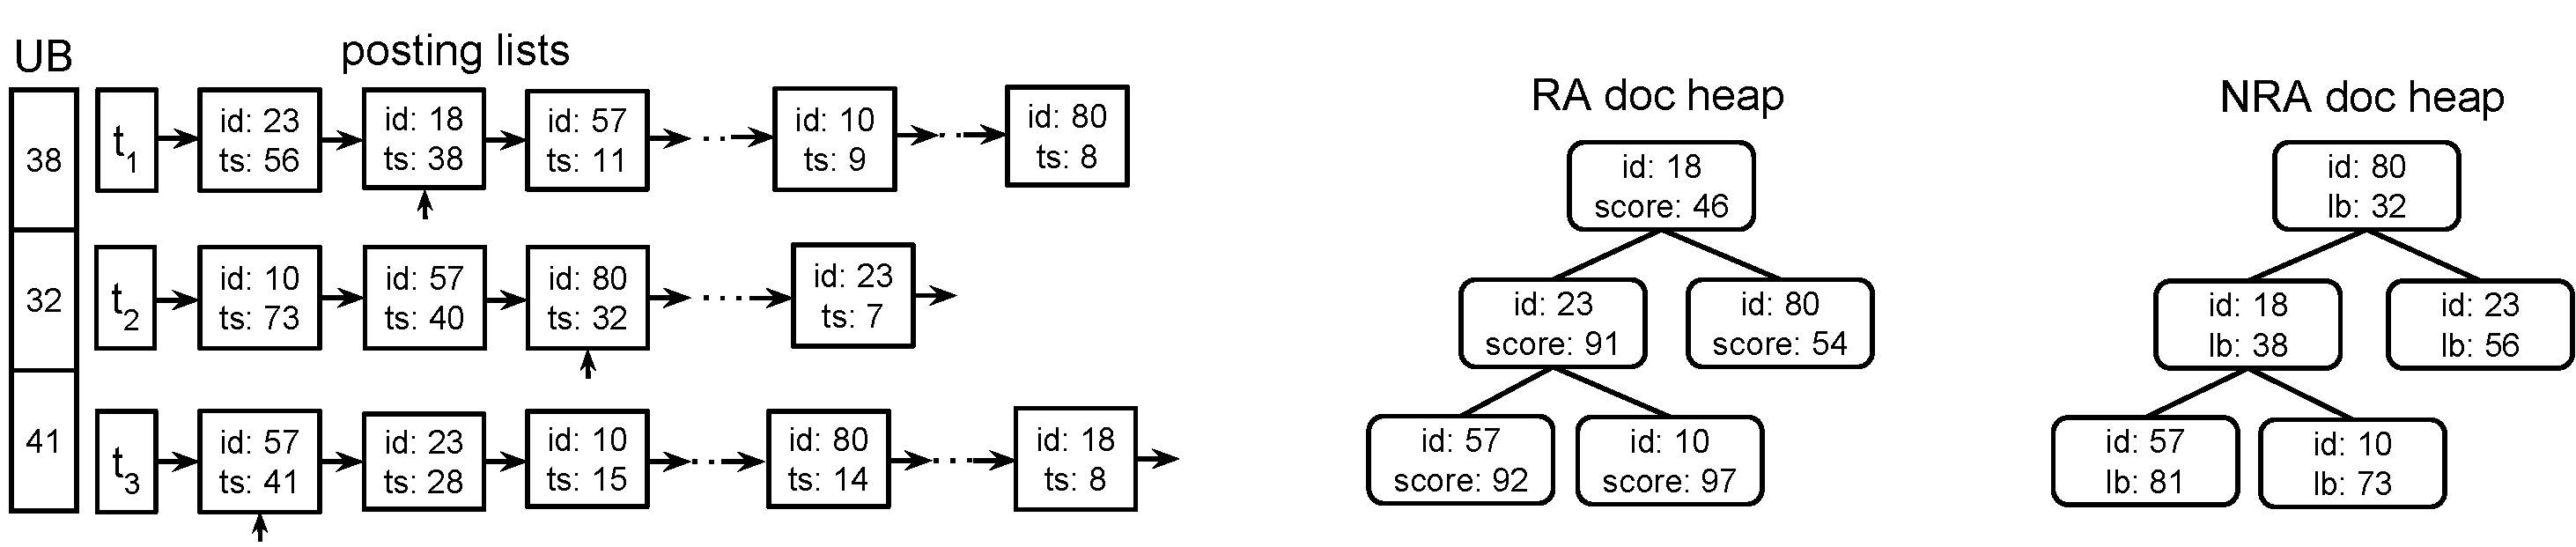
\includegraphics[width=\linewidth]{figures/postingsLists}
\caption{Traversal example in  RA and NRA variants of the Threshold Algorithm (TA). Posting lists are sorted by decreasing term score. Vertical arrows depict  iterator positions.  UB  holds upper bounds on the terms' contributions to scores of untraversed documents. The RA document heap is ordered by full document score, and the NRA heap  by partial score (lower bound).}
\label{fig:lists}
\end{figure*}

%Additionally, and similarly to DAAT-based algorithms, 
TA also maintains a threshold $\Theta$, i.e., the score of the $k$-th document in the heap.
%DC, and an upper bound on all other candidate scores not yet encountered. 
It stops when no candidate can exceed the threshold score. 
Fagin et al.\ present two flavors of the algorithm, which we now describe.
%The algorithm comes in two flavors.

\subsubsection{Random Access (RA)} 
The RA variant assumes that given a document id, we can use random access in order to obtain all its term scores in order to compute its total score. It thus computes the full score for every document it encounters. If the score is higher than the threshold, it is inserted into the heap. Then, $\Theta$ and the corresponding term's UB are updated. The algorithm stops when 
the following \emph{upper bound stopping condition} holds:
\begin{equation} \label{eq:stop}
\RAStop \triangleq \sum_{i=1}^m UB[i] \le \Theta.
\end{equation}

At this point, no non-traversed document can achieve a high enough score to be included in the heap. RA's output is the set of documents in the heap, ordered by their scores.

RA is an exact  algorithm as it returns the top-k results. In our evaluation, we implement an approximate variant of RA by stopping whenever the heap does not change for some parameter $\Delta$ ms. 
Note that the Threshold Algorithm is amenable to such early stopping because it traverses posting lists in order of score. High scoring documents are likely to become evident early, and finding new high scoring documents becomes less and less likely as the algorithm progresses. This is in contrast with document-order algorithms like BMW, where finding high scoring documents remains equally likely throughout the execution.

\remove{
RA was shown to be \emph{instance-optimal} in~\cite{Fagin:2003}, namely, the number of times it accesses data items is asymptotically close the optimum for every problem instance. Nevertheless, this analysis assumes that all accesses to data items have the same cost. 
This assumption holds if full scoring information about all data items is available in RAM (and resides in cache), but does not hold  for big datasets. 
}
%that do not fit into RAM (at least as long as non-volatile storage hardware does not provide memory-speed random access).
Unfortunately, random access is costly,  in particular for large data sets that do not reside fully in RAM.
Whereas a sequential posting list traversal requires infrequent I/O (at the end of each data block) and exhibits cache-friendly locality of access,  each random document access entails an I/O request and a cache miss.  
RA has an additional drawback in the IR setting, as it needs to maintain a secondary index by document id in addition to the posting lists sorted by term score, which doubles its footprint. 

\subsubsection{No Random Access (NRA)} 
The alternative NRA method %scans the posting lists sequentially in an interleaved manner while avoiding random access. It
refrains from computing the full score for each traversed document, and instead
maintains lower and upper bounds for candidate documents based on {\em partially\/} computed scores. 
%DC It stops when the lower bound $\Theta$ on all candidates in the top-k heap is larger than the upper bounds of all other potential candidates. 
%In more detail, 
%NRA tracks the partial scores of the documents it encounters in the course of its traversal. 
For a document $D$ and a term $t_i$, we define the upper bound $UB(D, t_i)$ to be the term score $ts(D, t_i)$ if it has already been encountered, and otherwise $UB[i]$, which provides an upper bound on $t_i$'s term score. We similarly define its lower bound $LB(D, t_i)$ to be the term score if it is known, and zero otherwise. We then aggregate these scores to compute the document's upper and lower bounds:
\[
UB(D) \triangleq \sum_{i=1}^m UB(D, t_i) \ ; \  
LB(D) \triangleq \sum_{i=1}^m LB(D, t_i).
\] 
For example, in Figure~\ref{fig:lists}, $UB(D_{57}) = 38+40+41 = 119$ and $LB(D_{57}) = 40+41 = 81$, whereas its actual score  is $11+ 40+41 = 92$.

NRA maintains the top-k heap according to the document \emph{lower bounds}, and $\Theta$ holds the smallest value among them. 
Its output is the set of documents in the heap, sorted by LB.

NRA's safe variant stops when (1) the \RAStop\ stopping condition of RA holds, 
and (2) all the  visited documents that are not in the heap have \emph{upper bounds} lower than or equal to $\Theta$. These two conditions are complementary: (1) ensures that no non-traversed documents are among the final top-k, whereas (2) ensures the same for  traversed documents that are not among the current top-k. 
While NRA does return the exact top-k results, unlike RA, it does not necessarily preserve the order among them, since some returned documents may be partially scored. As in RA, the approximate variant  stops after the heap has not changed for $\Delta$ ms.

